\pagestyle{quadrado}
\label{quadrado}

\begin{textblock*}{5.625in}(0pt,0pt)%
\vspace*{-3.5cm}
\hspace*{-2.77cm}\includegraphics*[width=175.2mm]{./propagandas/QUADRADO.pdf}
\end{textblock*}

\pagebreak %ROTA DE FUGA, FÁBIO ZUKER

\begin{center}
\hspace*{.5cm}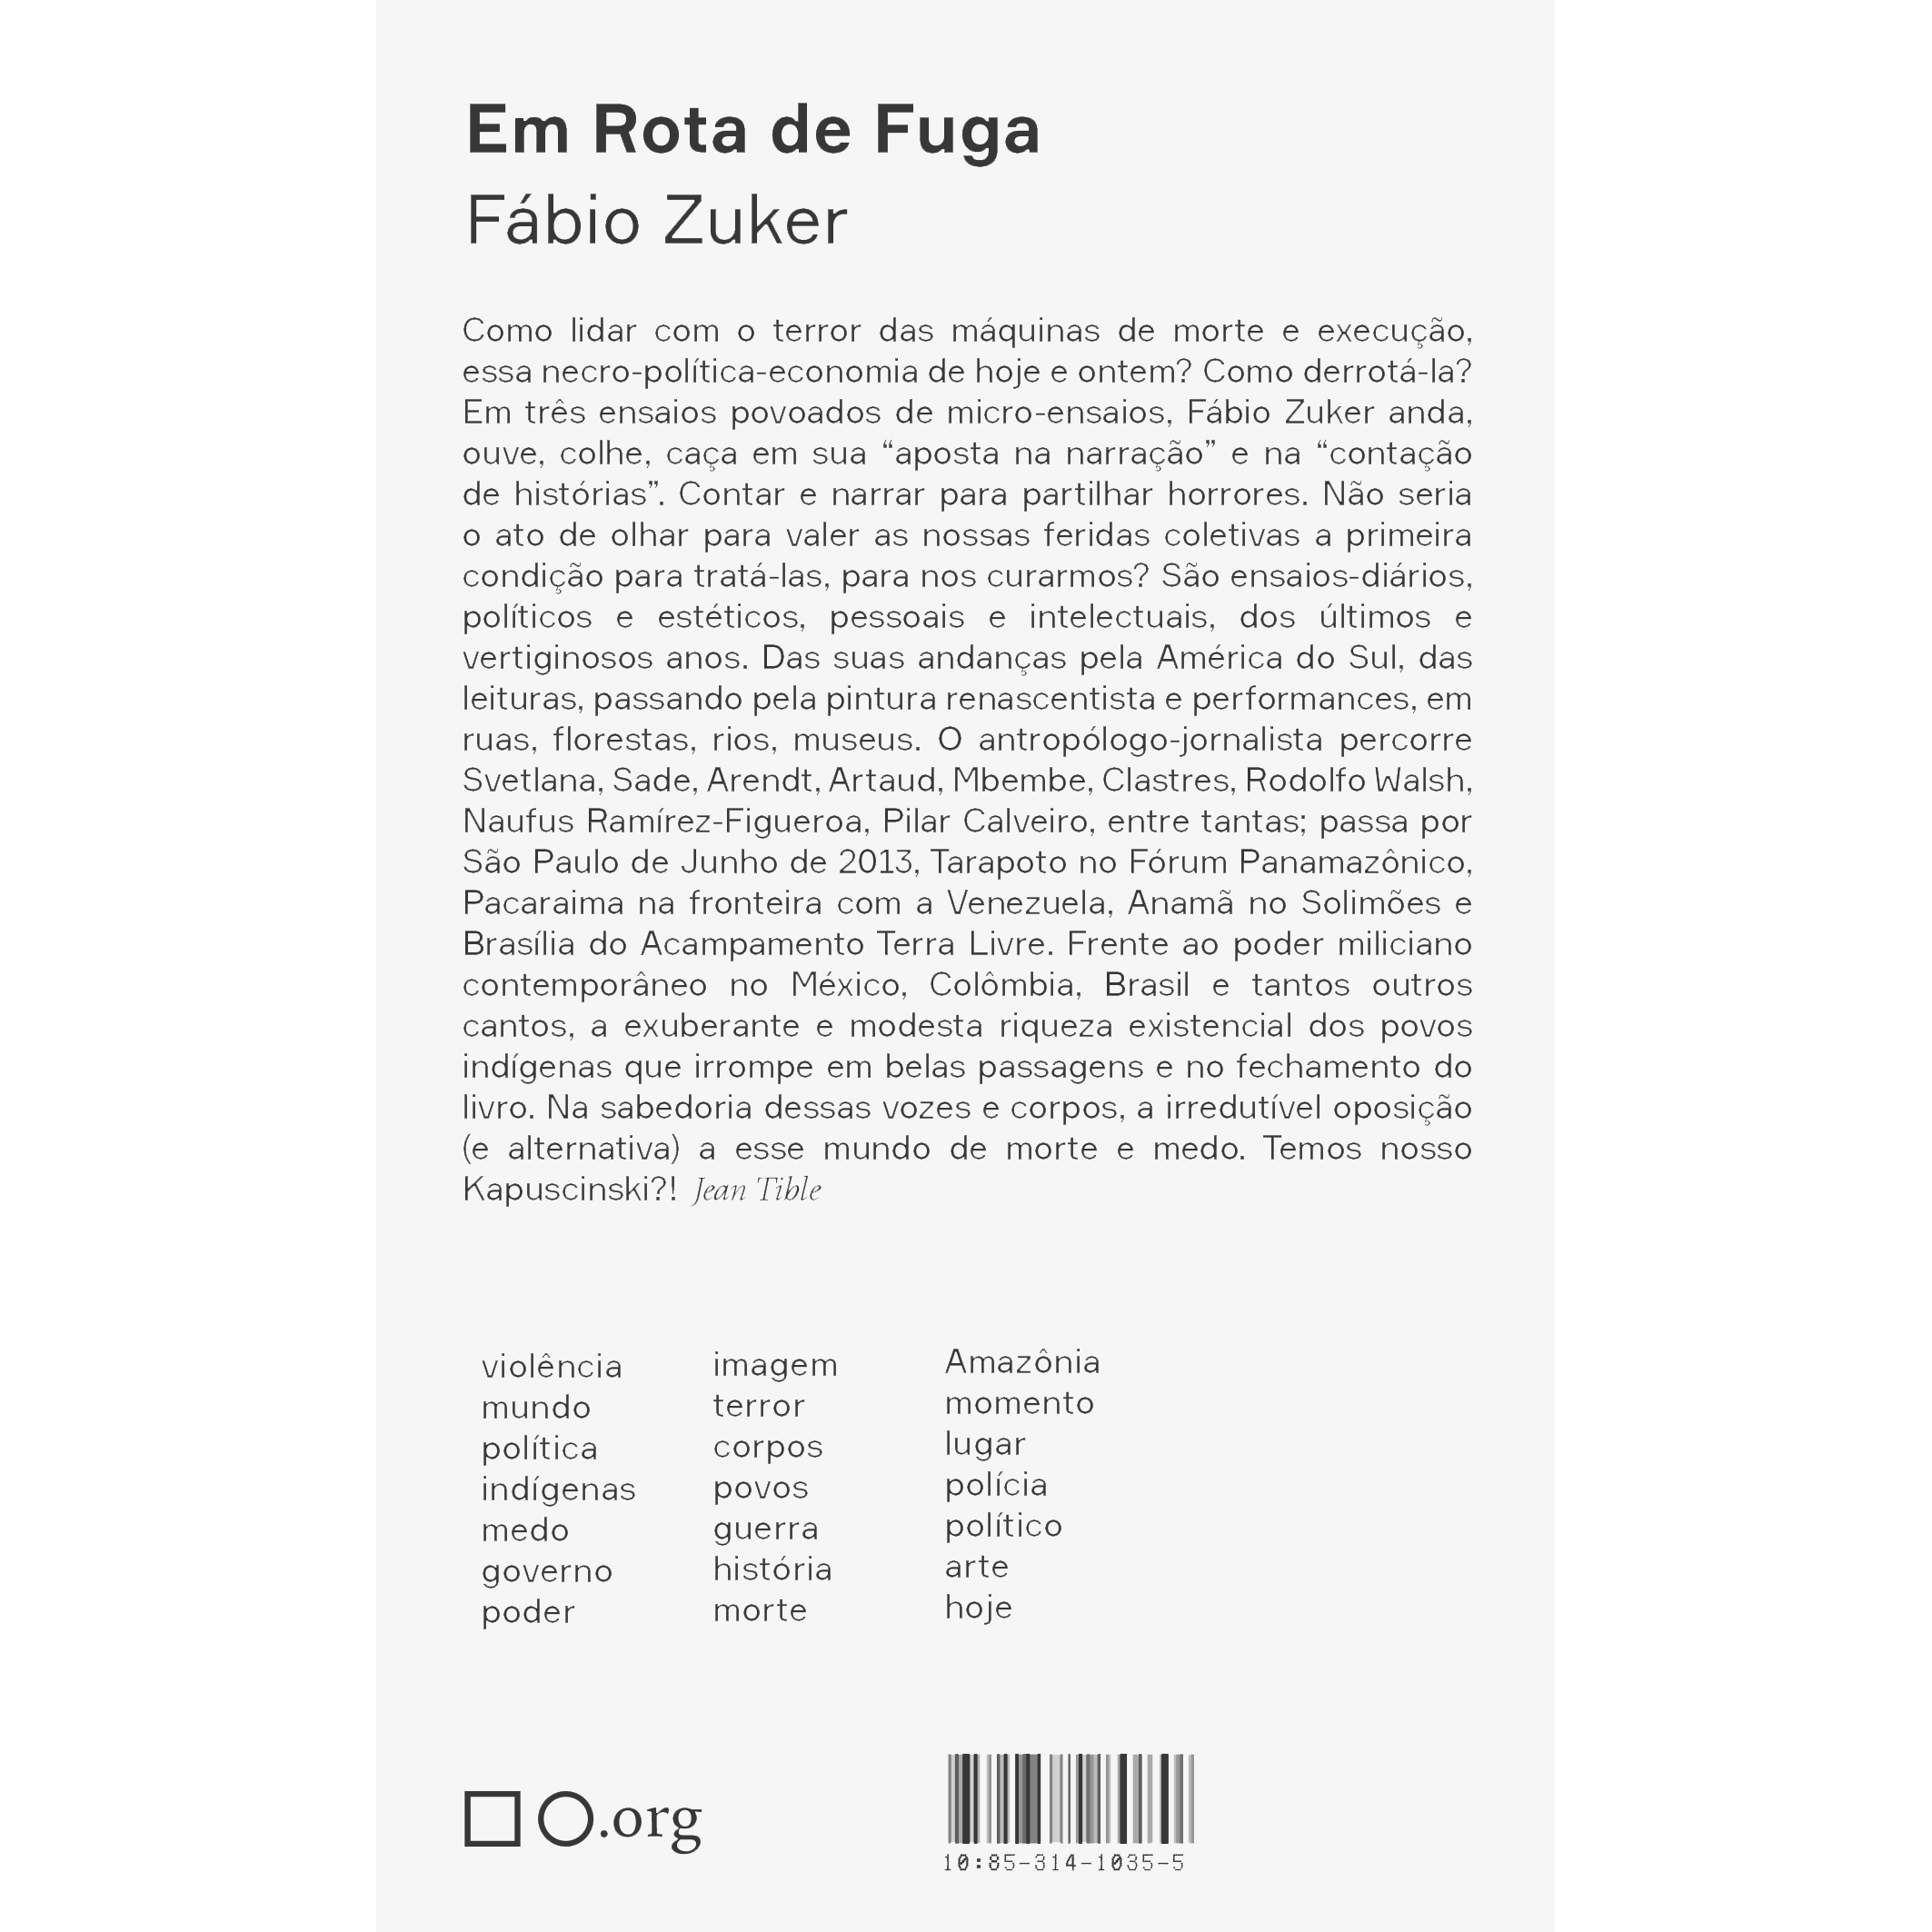
\includegraphics[width=74mm]{./grid/zuker.jpg}
\end{center}

\hspace*{-7cm}\hrulefill\hspace*{-7cm}

\medskip

\noindent{}O medo, em faceta promíscua aos mecanismos do governo neoliberal, é o fio condutor que percorre {\slsc{Em rota de fuga}}. Marcado por um olhar plurívoco, que perpassa a história da arte, Sade, cinema, vozes amazônicas e práticas de escrita contemporâneas, o escritor e antropólogo Fábio Zuker perscruta os desdobramentos dessa política para pensar outros mundos e formas de sensibilidade que criem efetivas rotas de fuga do círculo de violência neoliberal.

Ao tatear o “teatro"-peste” de Artaud enquanto político, analisar um quadro de Caravaggio ou abordar o medo do vazio que orientou o pensamento estético e político dos séculos passados, as reflexões do autor convergem para uma interrogação: \hlc[lightyellow]{a que servem as infinitas imagens de dor e violência diariamente veiculadas pela mídia? Como denunciar tais abusos e violências sem recorrer à megaexposição da morte}, como fazem de forma quase ritualística as milícias latino"-americanas? A escrita surge enquanto potência disruptiva para questionar os moldes do poder e suas discursividades.

\vfill

\hspace*{-.4cm}\begin{minipage}[c]{1\linewidth}
\small{
{\Formular{\textbf{
\hspace*{-.1cm}Editora: Quadradocirculo\\
Título: Em rota de fuga – ensaios sobre escrita, medo e violência\\
Autor: Fábio Zuker\\ 
ISBN: 978-85-7715-621-4\\
Páginas: 247\\
Formato: 11x18cm\\
Preço: R\$ 59,00\\
Disponibilidade: 14/08/2020
}}}}
\end{minipage}


\pagebreak %SALTO NO ESCURO, TUCA VIEIRA

\begin{center}
\hspace*{-3.6cm}\raisebox{5cm}{\rotatebox[origin=t]{90}{\huge\Formular{\textbf{Lançamento}}}}
\hspace*{3.1cm}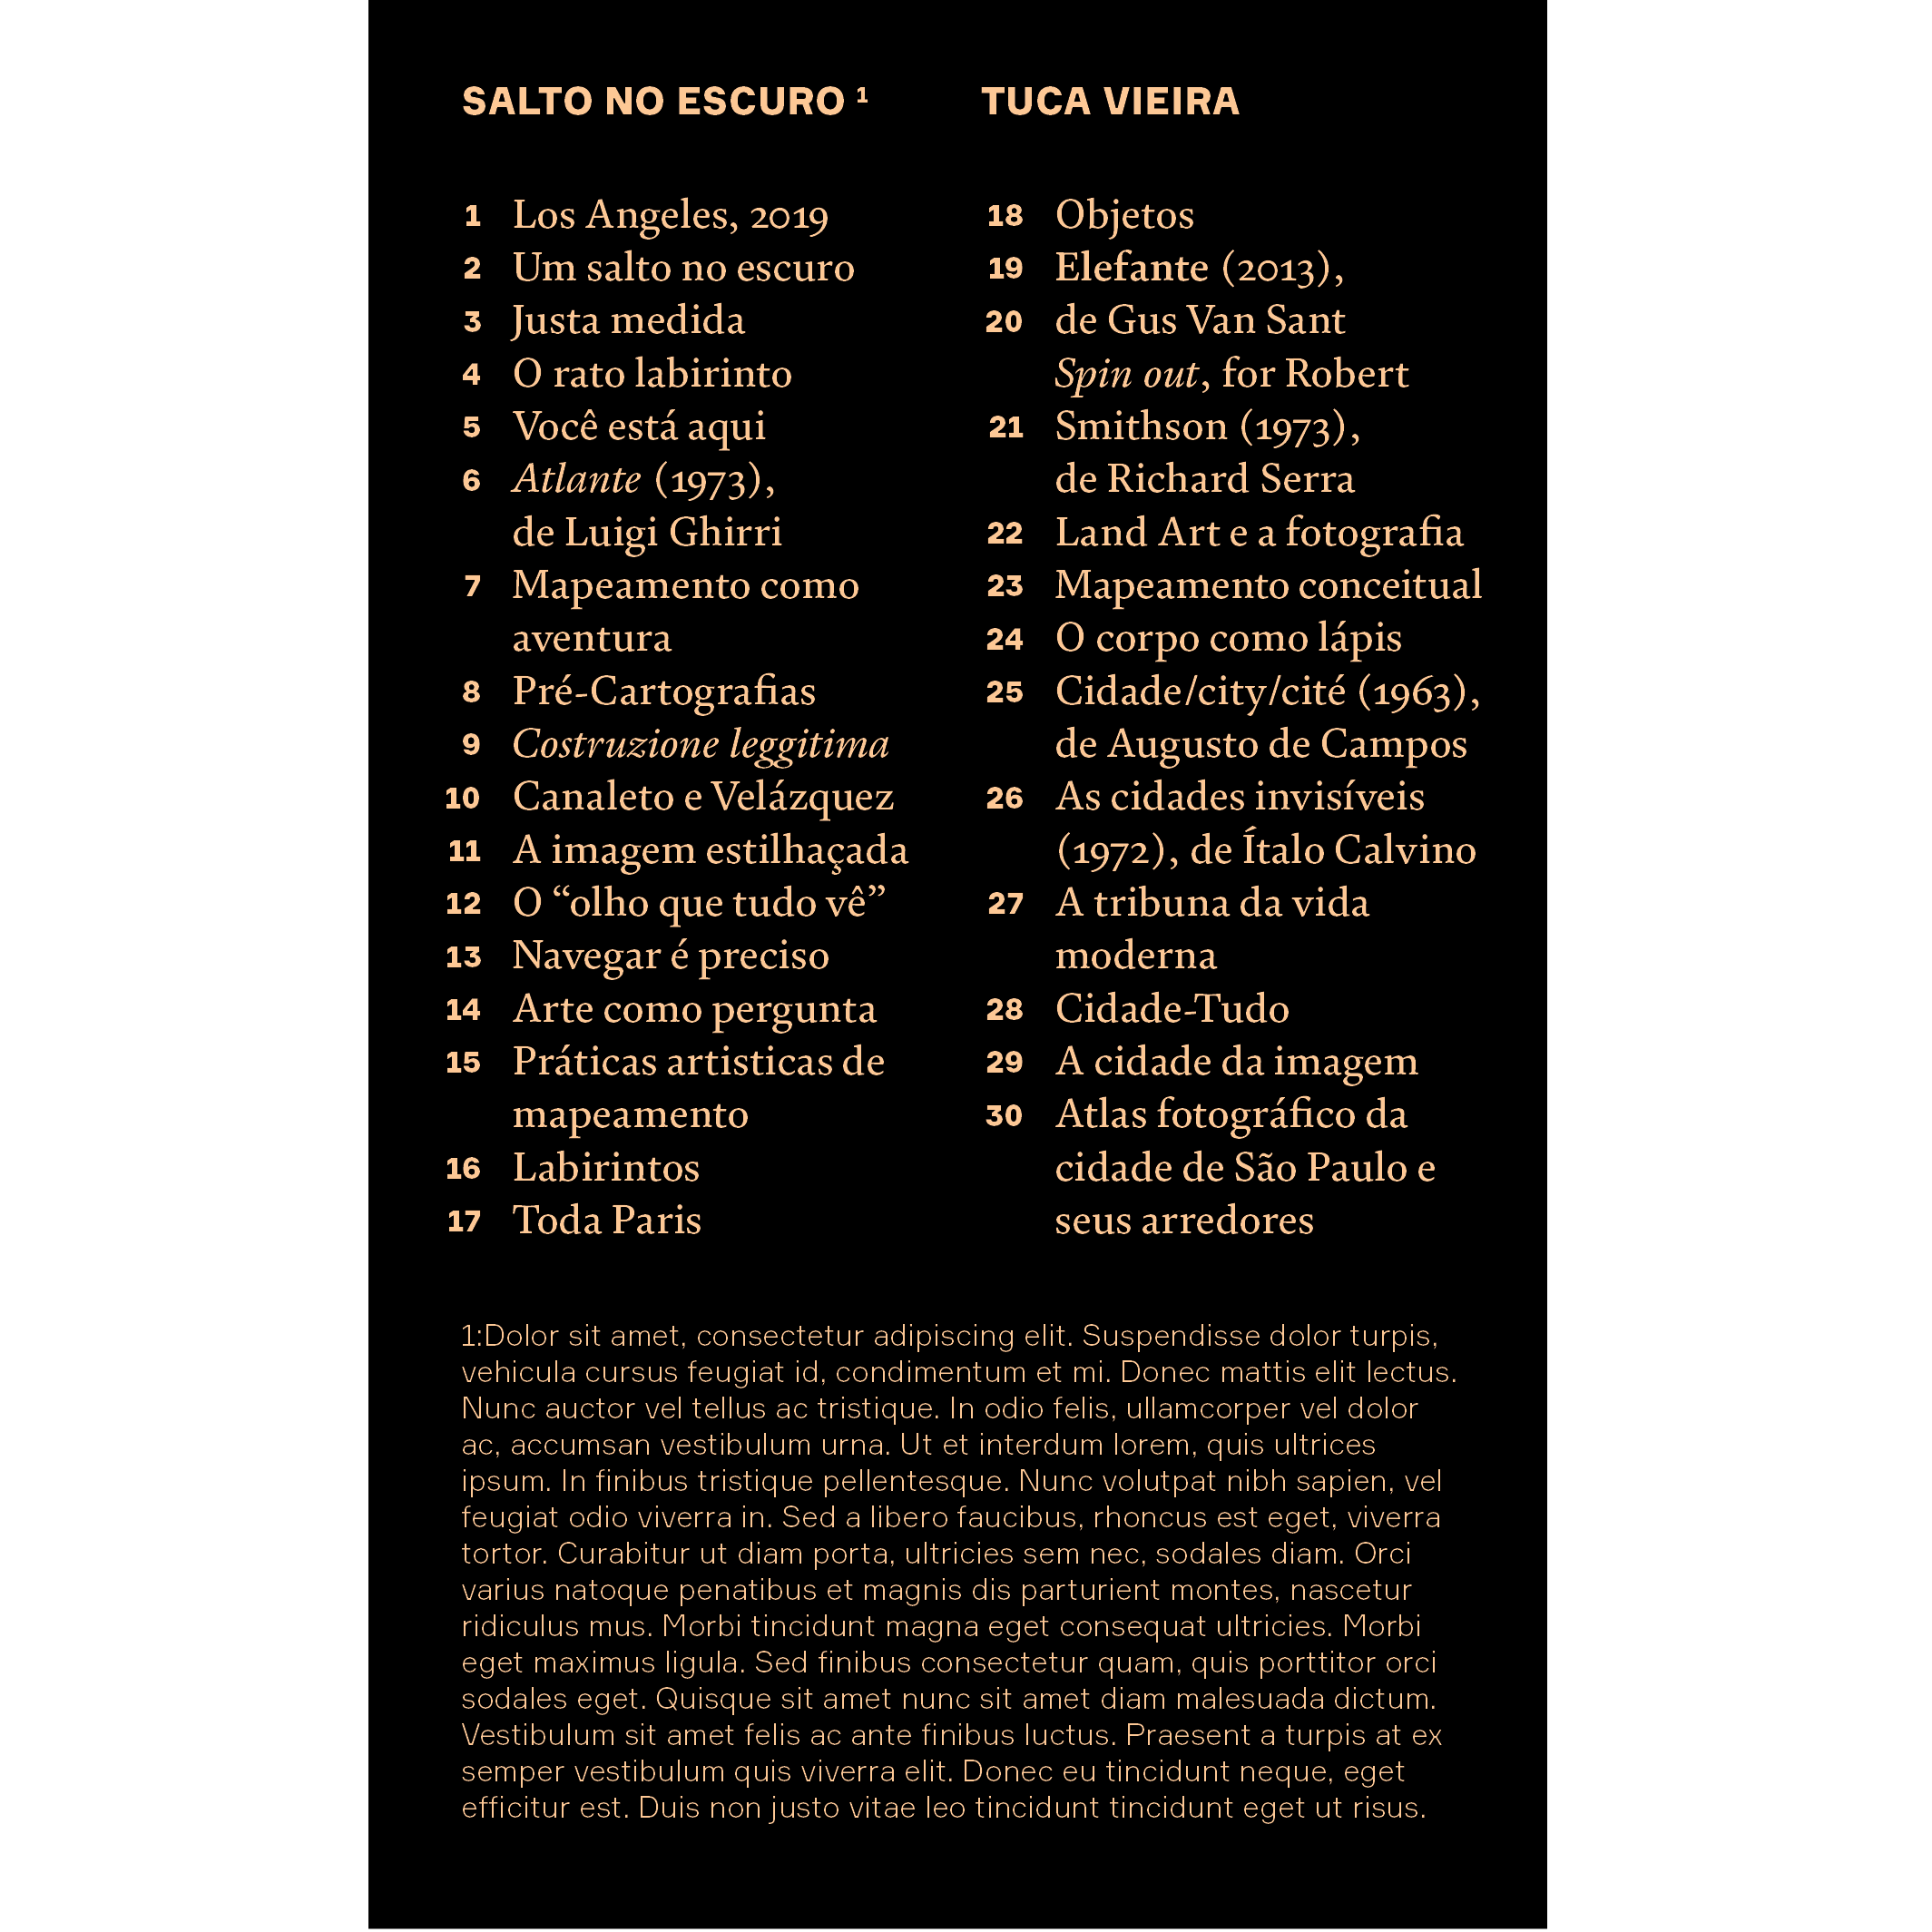
\includegraphics[width=74mm]{./grid/tuca.png}
\end{center}

\hspace*{-7cm}\hrulefill\hspace*{-7cm}

\medskip

\noindent{}Em um percurso que não deixa de ser um mapeamento afetivo do autor – com diversidade de referências literárias, cinematográficas, filosóficas, artísticas, históricas e arquitetônicas --- \hlc[lightyellow]{``Salto no escuro'' repensa criticamente as práticas de interação urbana, a partir de instigantes e assustadoras reflexões sobre as novas configurações espaciais das cidades.}

O renomado fotógrafo Tuca Vieira frequenta os mais díspares e múltiplos caminhos, centros urbanos, labirintos e criações artísticas, munido de arcabouço teórico e filosófico para análises precisas e necessárias sobre a cidade contemporânea e novas formas de interação humana. Diversas expressões artísticas se entrecruzam nesse percurso – de Borges, Kafka e Velázquez a William Gibson, os poetas concretistas e artistas da Land Art. Diante da vertiginosa aceleração da vida e inédita realidade impostas pela tecnologia, o autor instiga novas possibilidades e percepções diante de uma experiência progressivamente calculada e enquadrada virtualmente. 

\vfill

\hspace*{-.4cm}\begin{minipage}[c]{.5\linewidth}
\small{
{\Formular{\textbf{
\hspace*{-.1cm}Editora: Quadradocirculo\\
Título: Salto no escuro\\
Autor: Tuca Vieira\\ 
ISBN: 978-85-7715-622-1\\
Páginas: 500\\
Formato: 11x18cm\\
Preço: R\$ 99,90\\
Disponibilidade: 14/08/2020
}}}}
\end{minipage}

\pagebreak

\vspace*{1.5cm}

\noindent{}{\nohyphens{\LARGE{A história da arte e do mundo\\ como traço estético\\\noindent{}{\large\slsc{O medo do vazio emerge como princípio de um\\ espaço a ser preenchido, dominado, colonizado}}}}}

\bigskip

\hfill{}\scalebox{.8}{FÁBIO ZUKER}

\bigskip
\bigskip
\bigskip

\begin{multicols}{2}
{\slsc{Horror vacui}}, o horror ao vácuo, ou o medo do vazio, é um dos
princípios estéticos estruturantes do barroco e do rococó. Nenhum espaço
vazio, sem preenchimento por imagens e desenhos pode existir. Linhas,
traços, curvas e imagens devem ocupar, carregar, tornar o espaço cheio,
repleto, maciço, apinhado, opressivo. Como traço estético, a história da
arte está repleta de páginas acerca de sua origem céltica, islâmica,
bizantina ou mesmo viking.

\bigskip

{\small\fakereceipt{
“Talvez possamos aqui extrapolar o século XVII e a consolidação dos
impérios coloniais de Portugal e Espanha e o genocídio da população
ameríndia para pensar o próprio conceito de poder no Ocidente, formado à imagem
de um todo a ser preenchido”
}}

\bigskip

Mas foi ao longo do século \scalebox{.8}{XVII} que o {\slsc{horror vacui}} tornou"-se mais
influente, senão mesmo preponderante, na produção artística da Europa
Ocidental. Sempre me pareceu curioso que esse conceito estético tenha se
desenvolvido concomitante à expansão colonial europeia com a
estabilização dos impérios ultramarinos de Portugal e Espanha. Nada mais
significativo, nesse sentido, do que a produção de mapas do período, em
que todo espaço ``vazio'' é preenchido por textos, imagens de seres
imaginários, de sereias, de monstros ou de animais exóticos.

O horror ao vácuo, o medo do vazio, emerge como um princípio estético
conforme a um mundo a ser preenchido, dominado, colonizado. Um mundo em
que outros povos, outras formas de vida e de organização da vida comum
eram vistos pela Europa em expansão como definidos pela ausência:
selvagens sem cultura, política ou religião. Uma missão
civilizatória"-genocida de longa duração, empreendida pelos povos
europeus, objetivava preencher esse vazio constituinte do outro que, ao
ser dominado, passaria a ter religião, a ter leis e bons hábitos morais.
O outro como um vazio a ser preenchido à imagem de si, uma negação
absoluta da alteridade, que torna indistinguível etnocídio e genocídio.

Talvez possamos aqui extrapolar o século \scalebox{.8}{XVII} e a consolidação dos
impérios coloniais de Portugal e Espanha e o genocídio da população
ameríndia --- em 500 anos, estima"-se que 90\% da população foi exterminada
--- para pensar o próprio conceito de poder no Ocidente, formado à imagem
de um todo a ser preenchido. Uma concepção de poder dependente de uma
temporalidade específica, marcada por um destino manifesto de expansão.

A forma mais bem acabada, a concepção mais bem definida da potência
totalizante do poder foi elaborada
por uma filosofia/sociologia
política francesa ao longo da segunda metade do século \scalebox{.8}{XX}. Certamente
com objetivos críticos, elaborada por intelectuais militantes e em luta
por formas de emancipação coletiva, mas nem por isso imunes à sedução de
um conceito de poder com horror ao vazio, um poder que a tudo se aplica,
que tudo estrutura, que tudo domina e produz. O poder concebido como um 
espelho soberbo, que ao refletir a sua própria imagem em tudo, 
em tudo vê senão seu próprio reflexo.

Édouard Glissant, teórico martiniquenho, pensador da negritude e crítico
pós"-colonial analisa, em {\slsc{A poética da relação}}, essa afinidade
entre a estética e o colonialismo. Ambos são formas de ordenação do
mundo a partir de princípios hierárquicos já estabelecidos. Avessos à
desordem, à confusão e ao vazio, a colonização e a estética trazem em si
princípios organizacionais violentos. Em oposição à estética e sua forma
de organizar o mundo, Glissant propõe uma poética da relação, diversa,
emancipatória, alheia aos ditames da hierarquização, distante da imagem
de um poder totalizante.

Outra obra interessante é a da escritora norte"-americana Susan Sontag. 
Em seu ensaio {\slsc{Contra a
interpretação}}, a escritora elabora 
uma teoria"-prática da apreciação estética
anti"-interpretativista, que consiste menos em buscar o que uma
determinada obra de arte quer dizer, ou o que ela possa significar, e
mais o que ela faz, como nos toca, como nos afeta. Elabora uma
eroticidade da arte, sensível, epidérmica. Desloca o enfoque da
representação para a agência.

De alguma forma, tento me aproximar dessas pessoas, imagens, histórias,
livros ou obras de arte a partir de uma lógica estética da agência, do
que se produz. Estética na medida em que criam outros mundos, outras
formas de experiência e de sensibilidade, às quais cabe atentar. Efetivas rotas de fuga.

\bigskip

\noindent{}\textcolor{gray}{\footnotesize\slsc{Adaptado da introdução do livro “Em rota de fuga — ensaios sobre escrita, medo e violência”.}}
\end{multicols}
